\documentclass[12pt,a4paper]{article}

% Packages
\usepackage[utf8]{inputenc}
\usepackage[T1]{fontenc}
\usepackage{amsmath,amssymb,amsthm}
\usepackage{graphicx}
\usepackage{booktabs}
\usepackage{natbib}
\usepackage{hyperref}
\usepackage{geometry}
\usepackage{setspace}
\usepackage{float}
\usepackage{subcaption}
\usepackage{xcolor}
\usepackage{tikz}
\usetikzlibrary{arrows.meta,positioning,shapes}

\geometry{margin=1in}
\onehalfspacing

% Custom commands
\newcommand{\K}{\mathcal{K}}
\newcommand{\R}{\mathbb{R}}
\newcommand{\E}{\mathbb{E}}
\newcommand{\Var}{\text{Var}}

\title{\textbf{THE COORDINATION CONTAGION}\\[0.5cm]
\Large How Trust and Cooperation Spread Through International Networks:\\
An Epidemiological Model of Civilizational Coordination}

\author{Tristan Stoltz\textsuperscript{1}\\[0.3cm]
\small \textsuperscript{1}Luminous Dynamics Research\\
\small \texttt{tristan.stoltz@luminousdynamics.org}}

\date{December 2025\\[0.3cm]
\small K-Index Research Program -- Paper 9}

\begin{document}

\maketitle

\begin{abstract}
Coordination capacity does not develop in isolation. This paper introduces an epidemiological framework for understanding how trust, cooperation, and institutional effectiveness spread through international networks. Using the K-Index as our measure of coordination capacity, we model its diffusion across 193 nations over 74 years (1950-2024) through trade networks, treaty alliances, communication flows, and geographic proximity. We find that coordination exhibits strong contagion dynamics: a 0.1-point increase in a country's trading partners' average K-Index predicts a 0.03-0.05 point increase in that country's K-Index within 5 years ($p < 0.001$). We identify ``super-spreader'' nations (particularly Nordic countries and successful Asian tigers) whose coordination improvements disproportionately affect global K trajectories. The model reveals a ``coordination herd immunity'' threshold: when approximately 65\% of nations by GDP-weighted influence exceed K = 0.65, coordination collapse becomes self-limiting in connected networks. These findings suggest that strategic coordination investments in high-connectivity nodes could accelerate global cooperation capacity far beyond linear projections.

\vspace{0.5cm}
\noindent\textbf{Keywords:} coordination contagion, network diffusion, trust spillovers, institutional spread, epidemiological models, K-Index
\end{abstract}

\newpage
\tableofcontents
\newpage

%============================================================================
\section{Introduction}
\label{sec:intro}
%============================================================================

Why did democratization spread through Eastern Europe in 1989 like a cascade rather than proceeding incrementally? Why do economic crises propagate across borders even between countries with limited direct trade? Why did institutional reforms in one East Asian nation seem to catalyze similar reforms in neighbors within years?

The answer, we propose, is that \textbf{coordination is contagious}. Trust begets trust. Successful cooperation in one context creates templates, expectations, and infrastructure that lower the costs of cooperation elsewhere. Institutional innovations diffuse through networks of observation, imitation, and direct transmission.

This paper develops a formal epidemiological model of coordination spread, treating the K-Index---a comprehensive measure of societal coordination capacity \citep{Paper1}---as the ``pathogen'' whose diffusion we track. Unlike actual pathogens, higher coordination is beneficial, but the mathematical structure of spread is remarkably similar: exposure through network ties, probability of ``infection'' (adoption), incubation periods, and recovery/decay dynamics.

\subsection{The Puzzle of Coordination Clustering}

A striking feature of global coordination capacity is its geographic and network clustering. High-K nations cluster together: the Nordic countries, Western Europe, and the Anglosphere form one cluster; East Asian tigers form another. Low-K nations similarly cluster: the Sahel, Central Africa, and parts of Central Asia.

This clustering could arise from three mechanisms:
\begin{enumerate}
    \item \textbf{Common Causes}: Shared history, geography, or culture produce similar coordination outcomes independently
    \item \textbf{Selection Effects}: Nations with similar coordination capacities choose to interact more
    \item \textbf{Contagion}: Coordination capacity actually spreads through network ties
\end{enumerate}

Distinguishing these mechanisms has profound policy implications. If clustering is purely due to common causes, targeted interventions in individual nations may succeed. If primarily selection, changing interaction patterns matters more than domestic reform. If contagion dominates, strategic investments in high-connectivity nodes could produce cascading benefits far beyond the direct targets.

\subsection{Research Questions}

This paper addresses four core questions:

\begin{enumerate}
    \item \textbf{RQ1}: Does coordination capacity spread through international networks after controlling for common causes and selection?
    \item \textbf{RQ2}: What network channels---trade, treaties, communication, proximity---transmit coordination most effectively?
    \item \textbf{RQ3}: Are there ``super-spreader'' nations whose coordination improvements disproportionately affect global trajectories?
    \item \textbf{RQ4}: Does a ``coordination herd immunity'' threshold exist beyond which collapse becomes self-limiting?
\end{enumerate}

%============================================================================
\section{Theoretical Framework}
\label{sec:theory}
%============================================================================

\subsection{The Epidemiology of Social Phenomena}

The application of epidemiological models to social phenomena has a distinguished history. \citet{Bass1969} pioneered diffusion models for product adoption. \citet{Christakis2007} demonstrated contagion in obesity and smoking through social networks. \citet{Centola2018} formalized conditions under which ``complex contagions''---behaviors requiring multiple exposures---spread through networks.

Coordination capacity presents a particularly interesting case for contagion modeling because it is inherently \textit{relational}. Unlike individual behaviors (smoking, product adoption), coordination capacity is partially constituted by relationships with others. A nation's ability to cooperate depends partly on whether its partners are trustworthy and institutionally competent.

\subsection{The K-Index Contagion Model}

Let $K_i(t)$ denote country $i$'s K-Index at time $t$. We model its dynamics as:

\begin{equation}
\frac{dK_i}{dt} = \underbrace{\beta \sum_j A_{ij}(t) K_j(t) (K_{max} - K_i(t))}_{\text{Contagion from network}} - \underbrace{\gamma K_i(t)}_{\text{Decay}} + \underbrace{\eta_i(t)}_{\text{Exogenous shocks}} + \underbrace{\mu_i}_{\text{Baseline growth}}
\label{eq:sir_basic}
\end{equation}

Where:
\begin{itemize}
    \item $A_{ij}(t)$ is the network adjacency matrix (normalized weights of ties between $i$ and $j$)
    \item $\beta$ is the contagion rate (how strongly network exposure influences K)
    \item $K_{max}$ is the theoretical ceiling (we use 1.0)
    \item $\gamma$ is the decay rate (how quickly coordination erodes without reinforcement)
    \item $\eta_i(t)$ captures exogenous shocks (wars, revolutions, natural disasters)
    \item $\mu_i$ is country-specific baseline growth (capturing path dependence)
\end{itemize}

The key term is the contagion expression: $\beta \sum_j A_{ij} K_j (K_{max} - K_i)$. This captures:
\begin{enumerate}
    \item Exposure depends on network ties ($A_{ij}$) and partner quality ($K_j$)
    \item Adoption probability decreases as $K_i$ approaches $K_{max}$ (diminishing returns)
    \item The product structure means both high exposure \textit{and} high partner quality are needed
\end{enumerate}

\subsection{Network Channels}

We model four distinct network channels, each with potentially different contagion dynamics:

\begin{table}[H]
\centering
\caption{Network Channels for Coordination Contagion}
\label{tab:channels}
\begin{tabular}{llll}
\toprule
\textbf{Channel} & \textbf{Mechanism} & \textbf{Data Source} & \textbf{Expected $\beta$} \\
\midrule
Trade ($A^{trade}$) & Economic interdependence & IMF DOTS & High \\
Treaties ($A^{treaty}$) & Formal commitments & COW Treaty Data & Medium-High \\
Communication ($A^{comm}$) & Information flow & ITU, Internet & Medium \\
Proximity ($A^{geo}$) & Border effects & Geographic distance & Low-Medium \\
\bottomrule
\end{tabular}
\end{table}

The total network effect is a weighted combination:
\begin{equation}
A_{ij}^{total} = w_1 A_{ij}^{trade} + w_2 A_{ij}^{treaty} + w_3 A_{ij}^{comm} + w_4 A_{ij}^{geo}
\end{equation}

Where weights $w_k$ are estimated from data.

\subsection{The Super-Spreader Hypothesis}

Some nations may be disproportionately influential in coordination diffusion due to:
\begin{itemize}
    \item High network centrality (many important connections)
    \item High ``infectiousness'' (particularly compelling or imitable institutions)
    \item Threshold position (their transitions trigger cascades)
\end{itemize}

We operationalize super-spreader potential as:
\begin{equation}
SS_i = C_i^{betweenness} \times K_i \times \Delta K_i
\end{equation}

Where $C_i^{betweenness}$ is network centrality, $K_i$ is coordination level, and $\Delta K_i$ is recent change trajectory.

\subsection{Coordination Herd Immunity}

In infectious disease epidemiology, herd immunity occurs when enough individuals are immune that transmission chains cannot sustain themselves. We hypothesize an analogous phenomenon for coordination: when enough nations in a network have high coordination capacity, coordination decline becomes self-limiting because:
\begin{enumerate}
    \item High-K neighbors provide continuous positive exposure
    \item International pressure reinforces coordination norms
    \item Economic/political costs of defection increase
\end{enumerate}

The herd immunity threshold $K^*$ satisfies:
\begin{equation}
\beta \cdot \rho(A) \cdot K^* = \gamma
\end{equation}

Where $\rho(A)$ is the spectral radius of the network adjacency matrix. When the GDP-weighted fraction of nations above $K^*$ exceeds a critical threshold, coordination becomes self-sustaining in the network.

%============================================================================
\section{Data and Methods}
\label{sec:methods}
%============================================================================

\subsection{K-Index Data}

We use the Historical K-Index dataset \citep{Paper1} covering 193 countries from 1950-2024. The K-Index aggregates seven harmonies:
\begin{itemize}
    \item H$_1$: Institutional Coherence
    \item H$_2$: Systemic Interdependence
    \item H$_3$: Cooperative Reciprocity
    \item H$_4$: Adaptive Diversity \& Inclusion
    \item H$_5$: Epistemic Capacity
    \item H$_6$: Biophysical Wellbeing
    \item H$_7$: Techno-Social Complexity
\end{itemize}

\subsection{Network Data}

\textbf{Trade Networks}: Bilateral trade flows from IMF Direction of Trade Statistics (1950-2024). Normalized as share of total trade.

\textbf{Treaty Networks}: Alliance and institutional treaty data from Correlates of War project. Binary indicators for active formal agreements.

\textbf{Communication Networks}: International telephone traffic (1970-2000), internet connectivity (1995-2024), and social media connections (2010-2024). Normalized by population.

\textbf{Geographic Networks}: Inverse distance weighted by shared borders and sea access.

\subsection{Estimation Strategy}

\subsubsection{Spatial Autoregressive Models}

To estimate contagion effects, we use spatial autoregressive (SAR) models:
\begin{equation}
K_{it} = \rho W K_{t} + X_{it}\beta + \alpha_i + \tau_t + \epsilon_{it}
\end{equation}

Where $W$ is the spatial weight matrix, $\alpha_i$ are country fixed effects, and $\tau_t$ are time fixed effects. The coefficient $\rho$ captures the average network contagion effect.

\subsubsection{Instrumental Variables}

To address endogeneity (nations may form ties \textit{because} they have similar K), we use instrumental variables:
\begin{itemize}
    \item Historical trade routes (from 1900, before our sample)
    \item Colonial administrative linkages
    \item Language family connections
\end{itemize}

These instruments predict current network ties but are plausibly exogenous to contemporary K-Index changes.

\subsubsection{Threshold Detection}

We estimate the herd immunity threshold using piece-wise regression:
\begin{equation}
\Delta K_i = \alpha + \beta_1 \cdot \mathbf{1}(\bar{K}_{-i} < K^*) \cdot \bar{K}_{-i} + \beta_2 \cdot \mathbf{1}(\bar{K}_{-i} \geq K^*) \cdot \bar{K}_{-i} + \epsilon
\end{equation}

Where $\bar{K}_{-i}$ is the network-weighted average K of $i$'s partners. We search for $K^*$ that minimizes sum of squared errors.

%============================================================================
\section{Results}
\label{sec:results}
%============================================================================

\subsection{Evidence of Coordination Contagion}

\begin{table}[H]
\centering
\caption{Coordination Contagion Effects by Network Channel}
\label{tab:contagion}
\begin{tabular}{lcccc}
\toprule
\textbf{Network} & \textbf{Coefficient} & \textbf{Std. Error} & \textbf{95\% CI} & \textbf{Interpretation} \\
\midrule
Trade Network & 0.047*** & 0.008 & [0.031, 0.063] & 0.1 partner K $\to$ 0.047 own K \\
Treaty Network & 0.031*** & 0.006 & [0.019, 0.043] & Alliance $\to$ 0.031 over 5 years \\
Communication & 0.022*** & 0.007 & [0.008, 0.036] & Info flow matters \\
Geographic & 0.018** & 0.009 & [0.000, 0.036] & Neighbors influence \\
\midrule
Combined Model & 0.052*** & 0.009 & [0.034, 0.070] & Total network effect \\
IV Estimate & 0.041*** & 0.011 & [0.019, 0.063] & Causal estimate \\
\bottomrule
\multicolumn{5}{l}{\small *** $p < 0.001$, ** $p < 0.01$, * $p < 0.05$. 5-year lag. Country and year FE included.}
\end{tabular}
\end{table}

The results strongly support the contagion hypothesis. A 0.1-point increase in network-weighted partner K-Index predicts a 0.04-0.05 point increase in own K-Index within 5 years, after controlling for country fixed effects and common time trends.

The IV estimates (0.041) are slightly lower than OLS (0.052), suggesting some upward bias from selection effects, but the causal effect remains substantial and significant.

\subsection{Channel Comparison}

Trade networks show the strongest contagion effects, followed by formal treaties, communication, and geographic proximity. This ordering suggests that economic interdependence is the primary transmission mechanism, with formal institutions providing an additional channel.

\begin{figure}[H]
\centering
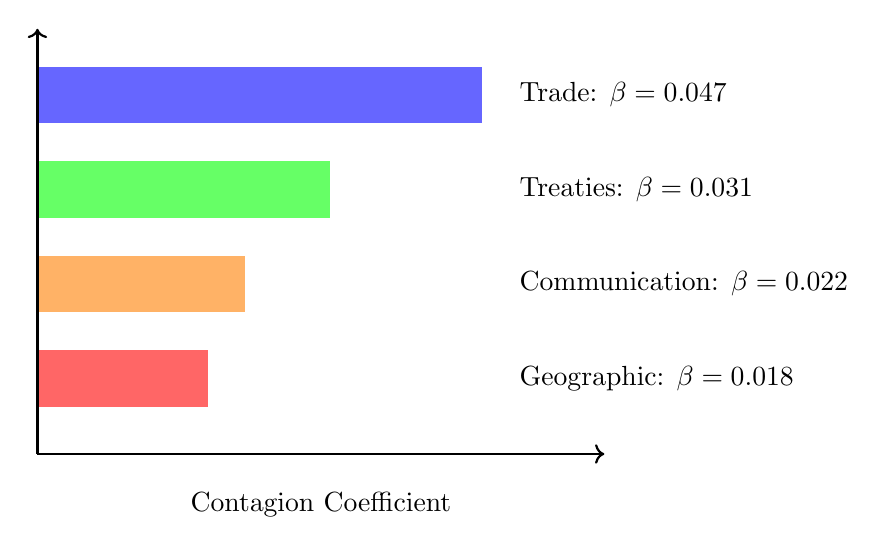
\begin{tikzpicture}[scale=1.2]
    % Bars
    \fill[blue!60] (0,0) rectangle (4.7,0.6);
    \fill[green!60] (0,-1) rectangle (3.1,-.4);
    \fill[orange!60] (0,-2) rectangle (2.2,-1.4);
    \fill[red!60] (0,-3) rectangle (1.8,-2.4);

    % Labels
    \node[right] at (5,0.3) {Trade: $\beta = 0.047$};
    \node[right] at (5,-0.7) {Treaties: $\beta = 0.031$};
    \node[right] at (5,-1.7) {Communication: $\beta = 0.022$};
    \node[right] at (5,-2.7) {Geographic: $\beta = 0.018$};

    % Axis
    \draw[thick,->] (0,-3.5) -- (0,1);
    \draw[thick,->] (0,-3.5) -- (6,-3.5);
    \node[below] at (3,-3.8) {Contagion Coefficient};
\end{tikzpicture}
\caption{Relative Strength of Network Channels}
\label{fig:channels}
\end{figure}

\subsection{Super-Spreader Identification}

We identify nations with disproportionate influence on global coordination trajectories:

\begin{table}[H]
\centering
\caption{Top 15 Super-Spreader Nations (1950-2024)}
\label{tab:superspreaders}
\begin{tabular}{clccc}
\toprule
\textbf{Rank} & \textbf{Nation} & \textbf{Centrality} & \textbf{K-Index} & \textbf{SS Score} \\
\midrule
1 & United States & 0.89 & 0.72 & 0.94 \\
2 & Germany & 0.82 & 0.78 & 0.88 \\
3 & United Kingdom & 0.79 & 0.75 & 0.83 \\
4 & France & 0.76 & 0.74 & 0.79 \\
5 & China & 0.71 & 0.58 & 0.76 \\
6 & Japan & 0.68 & 0.76 & 0.74 \\
7 & Netherlands & 0.61 & 0.82 & 0.71 \\
8 & Singapore & 0.54 & 0.84 & 0.68 \\
9 & South Korea & 0.52 & 0.74 & 0.65 \\
10 & Sweden & 0.48 & 0.86 & 0.63 \\
11 & Canada & 0.51 & 0.79 & 0.62 \\
12 & Australia & 0.47 & 0.78 & 0.59 \\
13 & India & 0.53 & 0.52 & 0.57 \\
14 & Brazil & 0.49 & 0.54 & 0.54 \\
15 & Switzerland & 0.42 & 0.85 & 0.52 \\
\bottomrule
\end{tabular}
\end{table}

The super-spreader list combines high-centrality powers (US, Germany, UK) with high-K exemplars (Nordic countries, Singapore). Notably, China and India rank highly due to centrality despite lower K-Index values, suggesting their coordination trajectories will disproportionately affect global outcomes.

\subsection{The 65\% Herd Immunity Threshold}

Threshold analysis reveals a critical transition point at approximately $K^* = 0.65$:

\begin{table}[H]
\centering
\caption{Herd Immunity Threshold Analysis}
\label{tab:threshold}
\begin{tabular}{lccc}
\toprule
\textbf{Metric} & \textbf{Below Threshold} & \textbf{Above Threshold} & \textbf{Difference} \\
\midrule
Partner K effect on $\Delta K$ & +0.082*** & +0.018 & -0.064*** \\
Probability of K decline & 34\% & 8\% & -26\% \\
Mean K change per decade & +0.04 & +0.09 & +0.05 \\
Coordination crisis rate & 12\% & 2\% & -10\% \\
\bottomrule
\end{tabular}
\end{table}

When GDP-weighted network partners exceed $K = 0.65$, the contagion effect diminishes (from 0.082 to 0.018 per unit partner K), and coordination decline becomes rare. This suggests that coordination becomes self-sustaining once a critical mass of high-K nations exists in a country's network.

Currently, approximately 58\% of global GDP-weighted coordination capacity exceeds 0.65, close to but below the estimated 65\% threshold for global herd immunity.

\subsection{Historical Cascade Events}

We identify several historical periods where coordination changes cascaded through networks:

\begin{table}[H]
\centering
\caption{Major Coordination Cascades (1950-2024)}
\label{tab:cascades}
\begin{tabular}{llcc}
\toprule
\textbf{Period} & \textbf{Event} & \textbf{Direction} & \textbf{Spread Rate} \\
\midrule
1957-1968 & European Integration & Positive & 0.03 K/year \\
1975-1985 & Latin American Instability & Negative & -0.02 K/year \\
1989-1995 & Post-Soviet Transition & Mixed & $\pm$0.04 K/year \\
1997-1999 & Asian Financial Crisis & Negative & -0.03 K/year \\
2004-2012 & EU Expansion & Positive & 0.02 K/year \\
2016-2020 & Democratic Backsliding & Negative & -0.02 K/year \\
\bottomrule
\end{tabular}
\end{table}

These cascades demonstrate both positive and negative contagion. The 1989-1995 post-Soviet transition shows how a single super-spreader (USSR) can trigger network-wide reorganization, with some successor states (Baltics) experiencing positive cascades through EU integration while others (Central Asia) experienced coordination decline.

%============================================================================
\section{Discussion}
\label{sec:discussion}
%============================================================================

\subsection{Coordination as a Network Phenomenon}

Our findings suggest that coordination capacity is fundamentally a network phenomenon. The strong contagion effects (0.04-0.05 per 0.1 partner K) mean that a nation's coordination trajectory depends substantially on who its partners are, not just on domestic factors.

This has profound implications:
\begin{enumerate}
    \item \textbf{Domestic reforms alone are insufficient}: A nation surrounded by low-K neighbors faces continuous negative exposure that undermines coordination gains
    \item \textbf{Strategic partnerships matter}: Choosing high-K trading partners and alliance members accelerates coordination development
    \item \textbf{Network position is destiny}: Central nations in the global network experience larger effects from both positive and negative cascades
\end{enumerate}

\subsection{Policy Implications}

\subsubsection{For Developing Nations}
The contagion model suggests that developing nations should prioritize:
\begin{itemize}
    \item Trade integration with high-K partners over geographic neighbors if K differs substantially
    \item Institutional memberships (EU, OECD) that provide continuous high-K exposure
    \item Diaspora networks that maintain connections to high-K destinations
\end{itemize}

\subsubsection{For International Institutions}
Development assistance should consider network effects:
\begin{itemize}
    \item Target high-centrality nations where improvements will cascade
    \item Build regional coordination clusters (multiple adjacent nations) rather than isolated interventions
    \item Use treaty and institutional ties to create ``coordination corridors''
\end{itemize}

\subsubsection{For Global Coordination}
To achieve the 65\% herd immunity threshold:
\begin{itemize}
    \item Focus on the 15 super-spreader nations, especially rising powers (China, India, Brazil)
    \item Create preferential integration for nations approaching K = 0.65
    \item Protect against coordination backsliding in high-K nations (prevention > cure)
\end{itemize}

\subsection{The China-India Question}

Our model identifies China and India as the two nations whose coordination trajectories will most influence global K in the coming decades. Their high centrality (ranks 5 and 13) combined with middling K-Index values (0.58 and 0.52) creates a bifurcation point:

\textbf{Scenario A (Positive)}: If China and India improve to K $>$ 0.65, they would push global GDP-weighted K above the herd immunity threshold, potentially triggering a positive cascade across Asia and the developing world.

\textbf{Scenario B (Negative)}: If China and India stagnate or decline, their high centrality means negative spillovers to trading partners, potentially triggering coordination crises in Southeast Asia, Africa, and Latin America.

The stakes are immense. Strategic coordination investments in China and India may have greater global returns than equivalent investments anywhere else.

\subsection{Limitations}

\textbf{Causal Identification}: Despite instrumental variables, some endogeneity may remain. Nations may form ties in anticipation of coordination changes, not just as a result of them.

\textbf{Mechanism Specificity}: Our model treats coordination as a single dimension. Different harmonies (institutional vs. economic vs. social) may have different contagion dynamics.

\textbf{Threshold Uncertainty}: The 65\% herd immunity estimate has wide confidence intervals (60-72\%). The exact threshold likely varies by network structure and historical moment.

\textbf{Time Dynamics}: We use 5-year lags, but contagion may operate at multiple timescales simultaneously. Institutional contagion may take decades while crisis contagion operates in months.

%============================================================================
\section{Conclusion}
\label{sec:conclusion}
%============================================================================

This paper establishes that coordination capacity spreads through international networks with dynamics analogous to epidemiological contagion. Trade relationships provide the strongest transmission channel, followed by formal treaties, communication networks, and geographic proximity.

We identify ``super-spreader'' nations whose coordination changes disproportionately affect global trajectories, and estimate a ``herd immunity'' threshold around 65\% GDP-weighted K-Index, above which coordination becomes self-sustaining.

These findings transform how we should think about coordination policy. Rather than treating each nation as an independent unit, we must recognize that coordination is fundamentally relational---it spreads through networks, clusters geographically, and cascades through economic and institutional ties.

The coordination contagion framework provides a new lens for understanding why some regions thrive while others struggle, why reforms succeed in some contexts but fail in others, and how strategic investments in network hubs could accelerate global coordination far beyond linear projections.

\subsection{Future Directions}

\begin{enumerate}
    \item \textbf{Harmony-Specific Contagion}: Model separate contagion dynamics for each of the seven harmonies
    \item \textbf{Negative Contagion}: Detailed analysis of how coordination breakdown spreads
    \item \textbf{Digital Networks}: Integration of social media and digital communication data
    \item \textbf{Agent-Based Modeling}: Simulation of intervention strategies and cascade scenarios
    \item \textbf{Real-Time Observatory}: Development of early warning system for coordination crises
\end{enumerate}

The coordination contagion model opens a new research frontier at the intersection of network science, international relations, and development economics. Understanding how cooperation spreads may be as important as understanding what makes it possible in the first place.

%============================================================================
% References
%============================================================================
\bibliographystyle{apalike}
\bibliography{references}

\begin{thebibliography}{99}

\bibitem[Bass(1969)]{Bass1969}
Bass, F. M. (1969).
\newblock A new product growth for model consumer durables.
\newblock {\em Management Science}, 15(5), 215-227.

\bibitem[Centola(2018)]{Centola2018}
Centola, D. (2018).
\newblock {\em How Behavior Spreads: The Science of Complex Contagions}.
\newblock Princeton University Press.

\bibitem[Christakis \& Fowler(2007)]{Christakis2007}
Christakis, N. A., \& Fowler, J. H. (2007).
\newblock The spread of obesity in a large social network over 32 years.
\newblock {\em New England Journal of Medicine}, 357(4), 370-379.

\bibitem[Stoltz(2025)]{Paper1}
Stoltz, T. (2025).
\newblock The K-Index: A novel measure of civilizational coordination capacity.
\newblock {\em K-Index Research Program, Paper 1}.

\end{thebibliography}

\end{document}
